%!TEX root = ../thesis.tex

\chapter[discussion]{Discussion}\label{chp:discussion}
% ~5 pages

The rapid progress of machine learning that started about a decade ago with the 2012 ImageNet competition and the work of \textcite{krizhevsky_imagenet_2012} all but slowed down during the course of this project. 
Following the papers by \textcite{choi_waic_2019,nalisnick_detecting_2019,hendrycks_deep_2019}, the field of out-of-distribution detection saw a surge of interest that has since grown yearly. Similarly, representation learning for speech has continued to advance with notable works such as CPC \parencite{oord_representation_2018}, wav2vec 2.0 \parencite{baevski_wav2vec_2020} and data2vec \parencite{baevski_data2vec_2022}. 

\moretodo{Adjust the below to include any discussion on out-of-distribution detection.}
Having examined VAEs and self"=supervised approaches for representation learning in \cref{part:unsupervised-uncertainty-estimation,part:unsupervised-speech-representation-learning}, in this discussion we will consider how VAEs might be enabled to learn representations more competitive with self"=supervised methods for downstream tasks (\cref{sec_discussion:representation-learning-with-vaes}). 
We will also complement the works on OOD detection in \cref{part:unsupervised-uncertainty-estimation}, which focused on image data, with a discussion about the OOD detection for audio and speech data (\cref{sec_discussion:out-of-distribution-detection-for-speech}). 
Since the work presented in \cref{part:medical-applications} only had limited focus on uncertainty, we will also present and discuss the use of calibration techniques for the stroke recognition model, drawing connections to how such systems might be perceived and used in practice (\cref{sec: discussion-stroke-recognition-uncertainty}). 

\section{Representation learning with variational autoencoders}\label{sec_discussion:representation-learning-with-vaes}
%
In this thesis we studied two different approaches to speech representation learning: VAEs in \cref{chp:paper-hierarchical,chp:paper-modelagnostic,chp:paper-brief,chp:paper-benchmarking} and self"=supervised methods in \cref{chp:paper-brief}. 
As we saw in \cref{chp:paper-hierarchical,chp:paper-modelagnostic}, the probabilistic formulation of VAEs provides benefits for their application to uncertainty quantification, although competitive methods based on self"=supervised foundation models have also been successful \parencite{xiao_we_2021,hendrycks_using_2019,bergman_classificationbased_2020}. 
Nonetheless, as discussed in \cref{chp:paper-brief}, self"=supervised methods are superior to VAEs when it comes to performance on most downstream tasks, such as speech recognition and spoken language understanding. 
While this statement of course depends on the task and the amount and type of unlabeled and labeled data, self"=supervised methods for speech are generally evaluated on downstream tasks that are harder and more complex than those used to evaluate VAEs. This is evidenced by the leaderboards on benchmarks such as SUPERB, SLUE and ZeroSpeech \parencite{yang_superb_2021,shon_slue_2021,dunbar_zero_2021}.\footnote{One example of comparable evaluation is that between \cref{tab: phoneme recognition (PER),tab:unsupervisedASR} where self"=supervised methods can be seen to outperform VAEs for phoneme recognition while self"=supervised methods are additionally reported for word-level speech recognition.} 
In the following, we will discuss potential directions of future research and try to shed light on why representations from VAEs underperform on downstream tasks and how they might be improved.


\subsection{Giving up?}

Two key observations might lead to the pessimistic view that VAEs are fundamentally unsuited for representation learning. 
First, VAEs are trained to maximize the ELBO which, when tight, is a marginal likelihood objective that is independent of the latent variables $\zb$. Second, as we saw in \cref{eq:variational-autoencoder-elbo-factorized-expected}, the ELBO can be written to reveal that its maximization leads to minimization of the mutual information between the observed and latent variables. In the following we will discuss each of these observations.

\paragraph{Marginal likelihood maximization} For any latent variable model $p_{\thetab}(\xb,\zb)$ we can use the posterior distribution $p_{\thetab}(\zb|\xb)$ to map a given observation $\xb$ to its latent representation $\zb$. We hope this representation is useful, for instance in the sense that it can improve performance on downstream tasks compared to other methods. Essential to the usefulness is the posterior distribution $p_{\thetab}(\zb|\xb)$. 

On the other hand, when we use maximum likelihood to train a latent variable model, we maximize the log-marginal likelihood $\log p(\xb)$. This can be equivalently phrased as maximizing the KL-divergence of the true data distribution $p_{\text{data}}(\xb)$ to the learned marginal, $D_{\mathrm{KL}}(p_{\text{data}}(\xb)\parallel p_{\thetab}(\xb))$.\footnote{%
Maximizing the likelihood $\sum_{n=1}^N \log p_\theta(\xb)$ w.r.t. parameters $\thetab$ is asymptotically equivalent to minimizing $D_{\mathrm{KL}}(p_{\text{data}}(\xb)\parallel p_{\thetab}(\xb))$: 
%
\begin{align}
    \argmin_\thetab D_{\mathrm{KL}}(p_{\text{data}}(\xb)\parallel p_{\thetab}(\xb)) 
    &= \argmin_\thetab \mathbb{E}_{p_{\text{data}}(\xb)} \left[ \log \frac{p_{\text{data}}(\xb)}{p_{\theta}(\xb)} \right] \nonumber \\
    % &= \argmin_\thetab \mathbb{E}_{p_{\text{data}}(\xb)} \left[ \log p_{\text{data}}(\xb) - \log p_{\theta}(\xb) \right] \nonumber \\
    &= \argmax_\thetab \mathbb{E}_{p_{\text{data}}(\xb)} \left[ \log p_{\theta}(\xb) \right] \nonumber \\
    &= \argmax_\thetab \lim_{n\rightarrow\infty} \underset{\text{log-likelihood}}{\underbrace{\sum_{n=1}^N \log p_{\theta}(\xb_n)}} \enspace . \nonumber
\end{align}
%
The last equality follows from the law of large numbers.
% \begin{align}
%     \mathcal{L}(\thetab; p_{\mathrm{data}}(\xb))
%     &= \lim_{N\rightarrow\infty} \frac{1}{N} \sum\limits_{n=1}^{N} \log p_{\thetab}(\xb) \\
%     &= \mathbb{E}_{p_{\mathrm{data}}(\xb)} \left[ \log p_{\thetab}(\xb) \right] \\
%     &= \mathbb{E}_{p_{\mathrm{data}}(\xb)} \left[ \log p_{\thetab}(\xb) - \log p_{\mathrm{data}}(\xb) + \log p_{\mathrm{data}}(\xb) \right] \\
%     &= \mathbb{E}_{p_{\mathrm{data}}(\xb)} \left[ \log p_{\mathrm{data}}(\xb) \right] + \mathbb{E}_{p_{\mathrm{data}}(\xb)} \left[ \log\frac{ p_{\thetab}(\xb)}{p_{\mathrm{data}}(\xb) }\right] \\
%     &= - \mathbb{H}[p_{\mathrm{data}}(\xb)] - D_\mathrm{KL}\left( p_{\mathrm{data}}(\xb)\mid\mid p(\xb) \right)
% \end{align}
} 
The first key observation then is that the marginal $p_{\thetab}(\xb)$, which we maximize, and the posterior $p_{\thetab}(\zb|\xb)$, which we want to produce useful representations, are separate properties of a latent variable model. Any combination uniquely defines a valid latent variable model. Hence, maximizing the marginal is a useless criterion for representation learning, regardless of the measure of usefulness \parencite{huszar_is_2017, alemi_fixing_2018}. 

VAEs, however, are not trained to directly maximize the marginal likelihood, but a lower bound of it, the ELBO,
%
\begin{equation} \label{eq:variational-autoencoder-elbo-factorized (discussion copy)}
    \mathcal{L}_{}(\xb;\thetab,\phib)
    = 
    \underset{\text{reconstruction loss}}{\underbrace{
        \mathbb{E}_{q_\phib(\zb|\xb)}\left[\log p_\thetab(\xb|\zb)\right]
    }}
     - 
    \underset{\text{KL-divergence to prior}}{
        \underbrace{\vphantom{\mathbb{E}_{q_\phib(\zb|\xb)}\left[\log p_\thetab(\xb|\zb)\right]}{D_\text{KL}\left( q_\phib(\zb|\xb) \parallel p(\zb) \right)}
    }} \enspace .
\end{equation}
%
Since the ELBO is not independent of the latent variables, its maximization will typically depend on the latent variables and the posterior $p(\zb|\xb)$. Nonetheless, being a lower bound of the marginal likelihood suggests it could suffer from similar issues under ``right'' conditions.


\paragraph{Mutual information minimization}
As we saw in \cref{subsec: mutual-information-interpretation-of-elbo}, optimizing the ELBO involves minimizing the mutual information between the latent and observed variables. We reprint equation \cref{eq:variational-autoencoder-elbo-factorized-expected} below for reference.
%
\begin{equation} \label{eq:variational-autoencoder-elbo-factorized-expected (discussion copy)}
    \mathbb{E}_{q_{\phib}(\xb,\zb)} \left[ \mathcal{L}_{}(\xb;\thetab,\phib) \right] = 
    \underset{\text{average reconstruction}}{\underbrace{
        \mathbb{E}_{q_{\phib}(\xb,\zb)}\left[ \log p_{\thetab}(\xb | \zb) \right]
    }}
    - 
    \underset{\text{marginal KL to prior}}{\underbrace{
    \vphantom{\mathbb{E}_{q_{\phib}(\xb,\zb)}\left[ \log p_{\thetab}(\xb | \zb) \right]}{
        D_{\mathrm{KL}}\left[ q_{\phib}(\zb) \parallel p(\zb) \right]
    }
    }} 
    -
    \underset{\text{mutual information}}{\underbrace{
    I_{q_{\phib}(\xb,\zb)}\left[\xb ; \zb \right]
    }} \. . \nonumber
\end{equation}
%
Note that we let $q_{\phib}(\xb,\zb) = q_{\phib}(\zb|\xb)\hat{p}(\xb)$ for ease of notation. 
% Optimizing the ELBO can be understood as simultaneously maximizing the average reconstruction likelihood, minimizing the marginal KL-divergence to the prior, and minimizing the mutual information between the observed and latent variables. 
We can see that optimizing the ELBO means learning a good one-to-one mapping from $\zb$ to $\xb$ (average reconstruction), fitting the aggregated posterior to the prior (marginal KL-divergence), while also not learning any stochastic dependency between $\xb$ and $\zb$ (mutual information). 
These objectives are conflicting and especially the minimization of mutual information seems counterproductive to our goal of learning useful representations \parencite{tomczak_trouble_2022}. 


\paragraph{How did this ever work?}

Even though these properties suggest that VAEs might not work well for representation learning, VAEs have consistently been shown to be able to learn meaningful representations \parencite{sonderby_ladder_2016,hsu_unsupervised_2017,maaloe_biva_2019,vahdat_nvae_2020,child_very_2021}. 
We can understand the reason for this by noting that both of the above scenarios can only occur if the optimization is sufficiently unconstrained. 

Specifically, the maximum marginal likelihood estimation in practice takes place not over all possible models, but over a constrained parametric class defined by the inference network $q_\phib(\zb|\xb) \approx p(\zb|\xb)$ and the generative model $p_\thetab(\xb,\zb) = p_\thetab(\xb|\zb)p(\zb)$. 
This introduces a coupling between the marginal $p_{\thetab}(\xb)$ and the posterior $p(\zb|\xb)$ which makes the maximum likelihood solution unlikely to correspond to completely useless representations \parencite{huszar_is_2017}. Particularly successful approaches have made this coupling stronger by sharing parameters between the inference and generative models \parencite{sonderby_ladder_2016,maaloe_biva_2019,vahdat_nvae_2020,child_very_2021}.
Similarly, maximizing the ELBO %in \cref{eq:variational-autoencoder-elbo-factorized-expected (discussion copy)} 
by exactly minimizing the mutual information term would correspond to a complete posterior collapse which necessitates a trade-off with the other terms. For a given model, this solution is almost surely a local minimum, and one that can often be avoided in practice. 
% Further evidence that the trouble is not solely attributable, the masked pre-training objective commonly used for self"=supervised methods has been shown to correspond to a maximum likelihood objective \parencite{moreno-munoz_masked_2023}.

Following this discussion, we can highlight the main challenges for VAEs to learn representations more competitive with self"=supervised methods. We must better understand how to impose constraints on the model class and optimization problem in a structured way in order to 1) ensure a strong coupling between the marginal likelihood and the usefulness of the posterior, and 2) make minimization of the mutual information term very difficult. In the following, we will discuss some possible approaches.

% + maximum likelihood does not guarantee good representations of unseen data. On the contrary; the two are actually only correlated by inductive biases present in the model type that we care about. 
% + VAEs do maximum likelihood.
%     + but this is true for any model trained with maximum likelihood
%     + in fact masked pre-trained used for many self-supervised methods can be seen as maximum likelihood training.

% + mutual information minimization of VAEs leads to difficulty of training and posterior collapse.
%     + only when properly constraining the inference and generative models do VAEs function.
%     + if the combined inference and generative models easily minimize the mutual information, while producing good reconstructions and making the marginal posterior match the prior, then the model will learn to disregard z, whatever is encoded in it. 
%     + this is especially prone to happen for strong generative models with those that are autoregressive on the observed variable as the core example. Since $p(\xb_t)$ in many cases can be modelled very well by a generative model of the form $p(\xb_t | \xb_{1:t-1})$, the potential improvement from using $p(\xb_t | \xb_{1:t-1}, \zb_{1:t})$, or even $p(\xb_t | \xb_{1:t-1}, \zb_{1:T})$, might be small compared to the magnitude of the mutual information term 
%     \cref{eq:variational-autoencoder-elbo-factorized-expected}


% \todo[inline]{Masked pre-training actually corresponds to marginal maximum likelihood optimization such as done by VAEs \parencite{moreno-munoz_masked_2023}. Since maximum likelihood in no way guarantees good representations, how do self"=supervised methods achieve  this, if they also do maximum likelihood?}


\subsection{Designing the latent space} 
Architectural improvements and hierarchies of latent variables are two related, and interesting, approaches to learning more semantic features in VAEs. 
Some success has been demonstrated in the image domain where models like BIVA \parencite{maaloe_biva_2019}, NVAE \parencite{vahdat_nvae_2020}, and VD-VAE \parencite{child_very_2021} use up to 78 stochastic layers and have achieved tight likelihoods and high-quality samples. 
Nonetheless, only limited effort has been put towards evaluating the usefulness for downstream task of representations learned by these very deep models. 
For speech, a hierarchical model operating on multiple temporal scales, such as the Clockwork VAE \parencite{saxena_clockwork_2021} adapted for speech in \cref{chp:paper-benchmarking}, might help better capture dependencies at longer ranges and encode more semantic features. 
For instance, phonetic content for pronunciation might be learned at lower layers, speaker identity at the upper layers, and semantic features, such as word-meaning, in between. 
Although some work has successfully separated speaker identity from content by modifying the latent variables and their dependencies \parencite{hsu_unsupervised_2017}, models that can learn a deep hierarchy of features for speech remains an open challenge. The work presented in \cref{chp:paper-benchmarking} represents an effort to make progress towards such a model, but more work remains.


\subsection{Adding a few labels} 
Another way to improve the representations learned in VAEs is via semi"=supervised learning. 
Here, a few labels are used to inform which patterns are learned from a large, mostly unlabeled, data set. 
This is usually done by defining a new stochastic variable as the target and deriving a semi-supervised version of the ELBO that accommodates using the labels when they are available, or marginalizing the target variable when they are not. The VAE is then trained on the labeled and unlabeled data simultaneously. 

Although VAEs are strong models for semi-supervised learning \parencite{kingma_semi-supervised_2014,kingma_improved_2016,maaloe_biva_2019}, self"=supervised methods have established themselves as superior for most tasks in this setting \cite{baevski_wav2vec_2020,jiang_speech_2021, liu_learning_2023}. 
Despite being theoretically appealing, joint objectives for semi-supervised learning in VAEs have practical drawbacks. By training on labeled and unlabeled data simultaneously, semi-supervised VAEs are often less flexible than self"=supervised methods which divide the training into two separate phases. By first fitting a general foundation model in an expensive pre"=training phase that can later be fine"=tuned, self"=supervised foundation models can be fine"=tuned for several downstream tasks, at relatively low cost. 
VAEs, on the other hand, must often learn the labeled downstream tasks while simultaneously training on the unlabeled data. This is computationally expensive, but also requires retraining with the unlabeled data, when new supervised data becomes available or a new task is added. Improvements in semi-supervised learning with VAEs might lead to more useful representations, but by requiring labels it remains less attractive than fully unsupervised learning.


\subsection{Approximating less}
VAEs are inherently approximate. Training is performed on a lower bound of the likelihood and inference is variational, amortized and for non-hierarchical models, mean field. As a consequence, the gradient itself is estimated inexactly, usually by only one posterior sample, leading to non-negligible variance. 
For that reason, it seems plausible that using tighter bounds and reducing gradient variance might indirectly yield more useful representations by improving learning in VAEs. 

Importance weighting the ELBO \parencite{burda_importance_2016} provides a tight bound on the likelihood, reduces gradient variance, and induces a complex implicit posterior distribution. 
Its use has become standard when reporting likelihood benchmarks but as we described in \cref{sec:variational-autoencoders}, \textcite{rainforth_tighter_2019} demonstrated that using it during training introduces high gradient variance for the inference network, hurting its ability to learn useful representations. However, Later works largely solved this issue and showed that the reduced variance leads to improved likelihoods \parencite{roeder_sticking_2017,tucker_doubly_2019,bauer_generalized_2021}. 

Despite much of this progress being prior to the latest, very large hierarchical VAEs, such as BIVA \parencite{maaloe_biva_2019}, NVAE \parencite{vahdat_nvae_2020}, and VD-VAE \parencite{child_very_2021}, these models are all trained with the single-sample ELBO using regularly reparameterized gradient estimator. Instead, these models rely on advanced inference networks \parencite{maaloe_biva_2019} and architectural improvements \parencite{vahdat_nvae_2020, child_very_2021} to overcome the challenges of training hierarchical VAEs. 
This indicates that there might be untapped potential in consolidating the work on low-variance gradient estimators, advanced architectures and inference methods, which could help improve representation learning in VAEs.


\subsection{Masking} 
As discussed in \cref{chp:paper-brief}, masking is one of the driving forces behind the success of self"=supervised methods for speech \parencite{devlin_bert_2018,baevski_wav2vec_2020}. By removing tokens from the input, or an early feature extraction layer, and tasking a model with inferring their representations, models are forced to learn how neighboring tokens relate to those that are masked. Depending on the size of the mask, these dependencies can be more or less semantic in nature. For instance, the wav2vec 2.0 model is well-known to learn representations that have high similarity with word identity and meaning \parencite{pasad_layerwise_2021}. 

In comparison, reconstruction in VAEs is done from latent variables that are inferred from the full, unmasked input. Since all information is generally available, this might allow the encoder and decoder models to perform well for reconstruction, even with no, or limited, use of contextual dependencies. Furthermore, VAE reconstruction almost always targets the direct input in order to learn the distribution over the training data and to enable generating new samples. However, compared to many self"=supervised methods that target intermediate, learned representations, this forces VAEs to encode all aspects of the input that are important to its representation in the observed space. As we saw in \cref{chp:paper-hierarchical}, this will generally include low-level features that are necessary for accurate input reconstruction. Such features require large latent space representations and model capacity \parencite{vahdat_nvae_2020,child_very_2021}, but are usually of lesser interest for downstream tasks \parencite{baevski_wav2vec_2020}.

Since the ELBO does not immediately allow for masking as part of the training, it has been only sparsely examined for VAEs. Specifically, masking has seen the most attention for VAEs within missing data imputation. In this setting, the input is partially observed, and often represented as a segmentation into observed and missing parts via a mask that indicates where the data is missing. The model is then trained to infer the latent variable from the observed data and reconstruction also deals only with the observed data. 
By comparison to self"=supervised approaches that use masking for representation learning, VAE training in the missing data setting focuses on reconstructing the observed data rather than the missing, which might not lead to the same benefits in representation learning. 
The idea of using VAEs to impute missing data was already examined in the seminal paper by \textcite{rezende_stochastic_2014}. Here the model was trained with fully observed data and used to impute data in an iterative sampling approach post hoc, leaving the learned representations unchanged.
Previous work that trains on partially observed data has largely focused on the ability of these models to yield high-quality imputations within the tabular and image data domains and have not probed for the effects on the learned latent representation \parencite{mattei_miwae_2019, ipsen_not-miwae_2021}. 

Including masked objectives into the principled probabilistic framework of VAEs might require rethinking the principles themselves. Nonetheless, relaxing the requirement of exact input reconstruction and enforcing the need for encoding (and decoding) contextual information is one of the strongest candidates to pave the way for future types of VAEs to learn representations that are competitive with self"=supervised methods.


\section{Out-of-distribution detection for speech}\label{sec_discussion:out-of-distribution-detection-for-speech}
%
% \moretodo[inline]{Out-of-distribution detection on speech?
%
% Outline:
% Intro paragraph drawing from OOD detection on images.
% Differences and unique challenges. Generally a harder problem than OOD detection for images
Somewhat casually ignoring the fact that this thesis is mainly interested in audio and speech data, the studies of \cref{part:unsupervised-uncertainty-estimation} dealt with OOD detection only in the context of image classification. The reason for this is that image classification has been the de facto standard task for benchmarking OOD detection methods since the first papers on the topic \parencite{choi_waic_2019,nalisnick_detecting_2019,hendrycks_deep_2019,kirichenko_why_2020}. 
In this section, we shall provide some perspective on OOD detection in the context of audio data. 

In certain cases, it might be possible to classify an image as OOD based only on the color or intensity of a single pixel. 
For most distributions, however, we are interested in a test that is sensitive to more semantic properties of the data - for instance the animal class, as discussed in the introduction (\cref{subsec:understanding-uncertainty}). 
For speech, this property holds too; a single amplitude value is unlikely to provide much information about the distributional origin of a speech sample. In fact, audio samples are one-dimensional which likely makes them even less discriminative compared to image pixels which generally have multiple channels e.g. for color. Instead, whether a sample is OOD must be inferred from correlations and patterns found in amplitudes along the temporal dimension. In this way, the task of OOD detection has a similar formulation across different data types. 

Nevertheless, few studies have explored OOD detection specifically for speech. 
In one recent study, the authors propose a supervised approach that uses a $k$NN classifier fitted to representations of the training data \parencite{bukhsh_outofdistribution_2023}. The approach is tuned to a fixed recall on the training data and operates on full length audio samples. This method is similar to image methods that fit a Gaussian mixture to an appropriate model layer \parencite{lee_simple_2018, xiao_we_2021}. In the early work of \textcite{hendrycks_baseline_2017}, the OOD detection method (based on softmax probabilities) is also benchmarked on audio datasets including TIMIT and Aurora-2 \parencite{garofolo_timit_1993,pearce_aurora_2000}. These works strongly suggest that with good data representations, we can use similar methods for OOD detection on both audio and images.

% - Harder to work with: Images provide immediate, human-interpretable feedback but audio requires playback which takes time.
% The studies on OOD detection for audio reflect its similarity to OOD detection for images. 
Despite the similarities of the OOD detection task and its methods between data types, audio comes with unique properties. 
Where images are immediately interpretable to a researcher by visual inspection, audio requires playback, often in real-time, to reveal its contents. This fact alone is likely to have reduced interest in audio data by simply making it more time-consuming to work with than images. On top of this, audio is generally variable length and requires more computer memory than images which increases complexity and the amount of compute required to obtain equivalent results compared to images. 
As such, audio-based OOD detection is likely to benefit from progress in standardized frameworks for machine learning like PyTorch \parencite{paszke_automatic_2017} and HuggingFace \parencite{wolf_huggingface_2020,lhoest_datasets_2021} which make it increasingly easier to work with irregular data types. 

% - Temporal scale, can be OOD in local segments but not entire sequence. 
Another fundamental difference between audio and images is that audio is additive; two signals can be added together to form a new, mixed signal that is meaningful in the sense that it might as well be a true recording. 
Addition of two images on the other hand produces an image that is not generally representative of what might be photographed. 
This property of images has led to the practice of evaluating OOD detection performance by comparing examples between different datasets (e.g. MNIST versus FashionMNIST). 
Interestingly, the additive property of audio allows complementing this dataset-versus-dataset evaluation with an approach where in-distribution examples are augmented to be OOD by mixing with unknown sources. This was initially explored by \textcite{hendrycks_baseline_2017} but has not seen a wide investigation. 

Finally, most work on OOD detection has focused on an example-centric approach where an entire example must be classified as either in- or out-of-distribution. 
For audio, however, it is easy to create examples where local segments are OOD while other parts are not. 
Using the additive property, we could add a loud Morse signal on top of a dialogue to change a segment of in-distribution audio to OOD. 
Similarly, silence might be used as a kind of padding to insert entirely OOD segments in between in-distribution parts without addition and without significant boundary effects. 
For images, the equivalent approach is similar to the successful regularization technique CutMix \parencite{yun_cutmix_2019} which pastes unrelated images into an example image. In the context of OOD detection, this approach creates strong boundary errors, which might be used or learned to easily detect such synthetic OOD images. 
Examples that contain locally OOD parts might occur naturally too; both in the image and audio domains. All kinds of unknown sound can be considered OOD and hence any recording might be locally OOD. In image segmentation, unknown object classes might similarly be seen as locally OOD parts of an example. Future research might examine further how detection of locally OOD examples differs from the dominant example-centric approach. 


% \section{\Cref{chp:paper-retrospective} revisited: Calibration}
\section{Uncertainty of the stroke recognition classifier} \label{sec: discussion-stroke-recognition-uncertainty}

Our work on stroke recognition in \cref{chp:paper-retrospective} focuses on the predictive performance of the ensemble model and an analysis of feature importance, but does not explicitly consider uncertainty estimation. 
As we discussed in \cref{subsec:model-calibration}, such a model can be calibrated to predict probabilities that are aligned with the empirical probability of the model being correct on some validation set. Here we present and discuss model calibration for the ensemble model. 

We compute the calibration curve by sorting the probabilities predicted on the test set into a number of bins spanning the range from zero to one. For each bin $b$, we compute the mean predicted probability $\bar{p}$ and the fraction of examples for which the model predicted correctly $r_{b}$. The calibration curve is the drawn from the $\{(\bar{p}_{b}, r_{b})\}_b$ pairs. For any given bin, a perfectly calibrated model would have the same fraction of correct predictions as that bin's mean value, $\bar{p}_{b} = r_{b}\,\forall\,b$. 

\begin{figure}[t!]
    \centering
    \begin{subfigure}[c]{0.49\columnwidth}
        \centering
        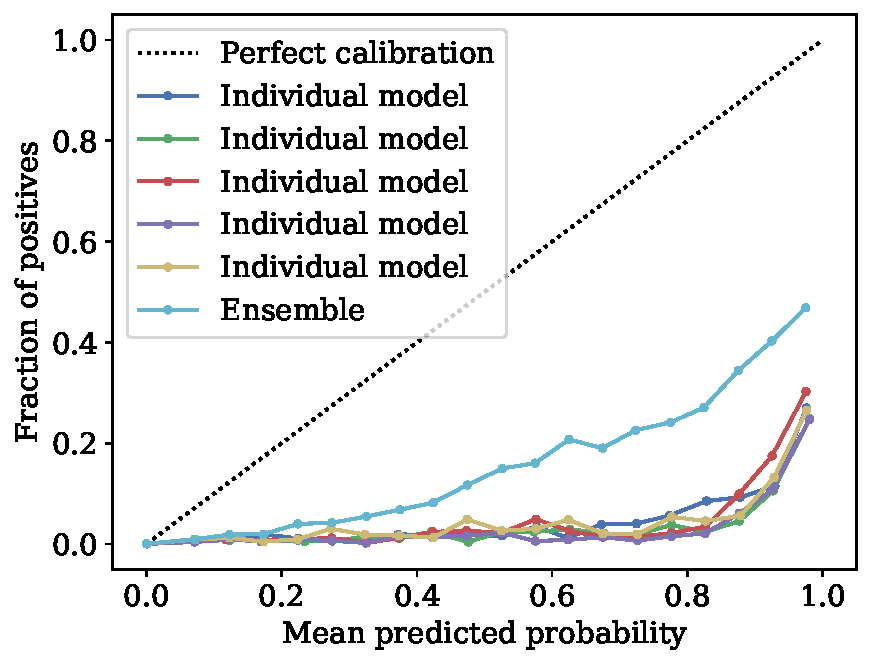
\includegraphics[width=1\columnwidth]{paper_retrospective_calibration_plots/calibration_curve_ensemble_and_all_models_uncalibrated.pdf}
    \end{subfigure}
    \hfill
    \begin{subfigure}[c]{0.49\columnwidth}
        \centering
        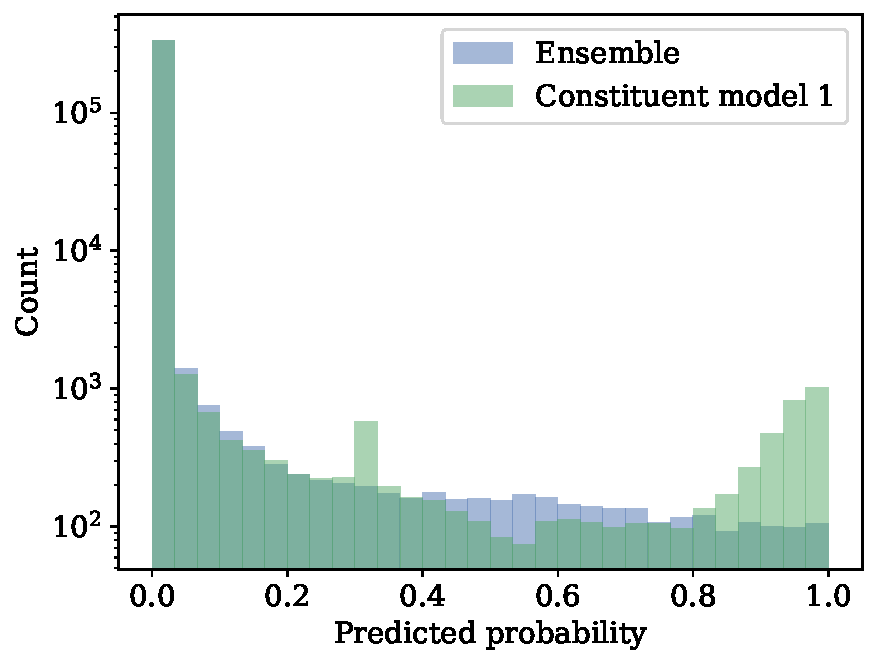
\includegraphics[width=1\columnwidth]{paper_retrospective_calibration_plots/histogram_ensemble_and_single_model.pdf}
    \end{subfigure}
    \caption[Calibration curve for the uncalibrated stroke recognition ensemble and empirical distribution of predicted probabilities.]{ Calibration curve for the uncalibrated stroke recognition ensemble (left) and the histogram of predicted probabilities (right) for the test set. We use the ensemble that achieved the median F1-score reported in \cref{fig_retrospective:figure1-roc-curve} and \cref{tab_retrospective:table3-occlusion-analysis}.}
    \label{fig_discussion:retrospective-paper-calibration-curve-of-uncalibrated-model}
\end{figure}

The calibration curve for the uncalibrated stroke recognition ensemble and its constituent models is plotted in \cref{fig_discussion:retrospective-paper-calibration-curve-of-uncalibrated-model} along with a histogram of its predicted probabilities. The miscalibration issue that we previously discussed is clearly visible as a strong overconfidence for both ensemble and constituents, although the ensemble is much better calibrated than its constituents. Since the ensemble's output probability is computed as the harmonic mean of the five constituent model probabilities, it can never exceed the maximum probability predicted between the constituent models. This property tends to make ensemble probabilities less extreme and, since the constituent models are overconfident, this results in better calibration. 

\begin{figure}[t!]
    \centering
    \begin{subfigure}[c]{0.49\columnwidth}
        \centering
        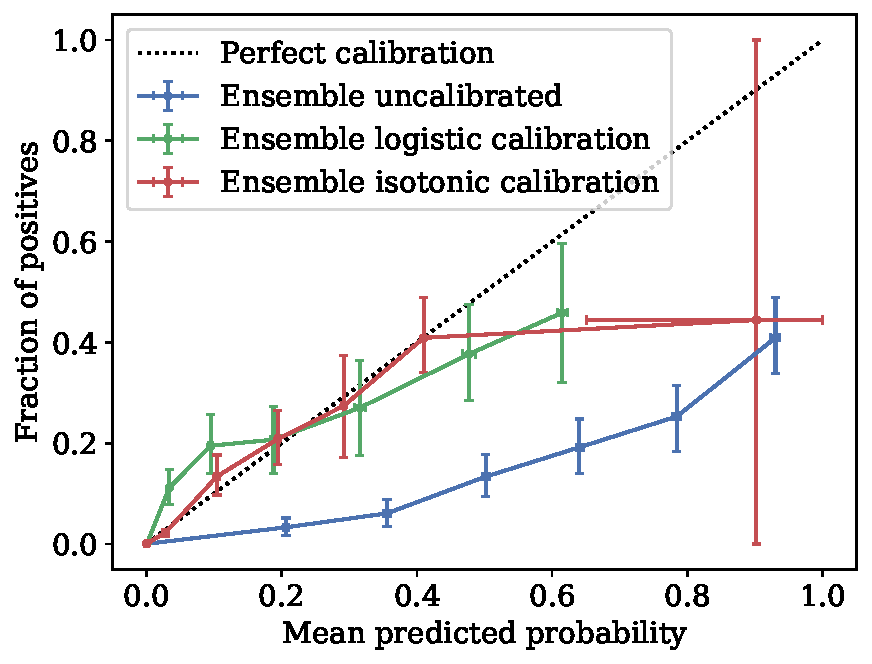
\includegraphics[width=1\columnwidth]{paper_retrospective_calibration_plots/calibration_curves_ensemble_with_cis.pdf}
    \end{subfigure}
    \hfill
    \begin{subfigure}[c]{0.49\columnwidth}
        \centering
        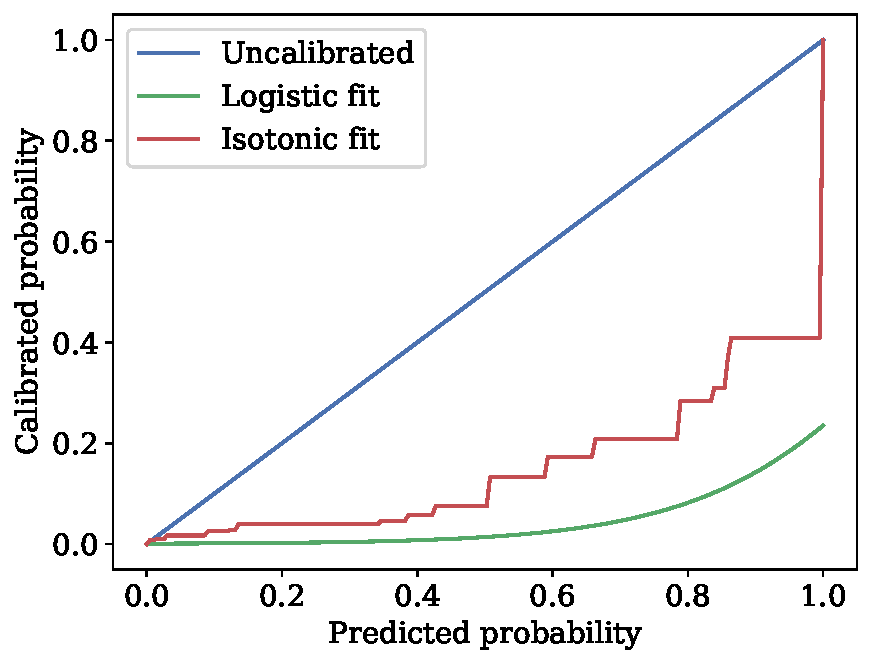
\includegraphics[width=1\columnwidth]{paper_retrospective_calibration_plots/calibration_fits_ensemble.pdf}
    \end{subfigure}    
    \caption[Calibration fits and curves for the stroke recognition ensemble using Platt-scaling and isotonic regression for calibration.]{ Calibration curves using sigmoid and isotonic calibration fits for the stroke recognition ensemble model (left) and the calibration fits (right) for the test set. We use the ensemble that achieved the median F1-score reported in \cref{fig_retrospective:figure1-roc-curve} and \cref{tab_retrospective:table3-occlusion-analysis}.}
    \label{fig_discussion:retrospective-paper-calibration-curve-sigmoid-isotonic}
\end{figure}

To calibrate the ensemble model, we can use methods such as Platt-scaling \parencite{platt_probabilistic_1999} or isotonic regression \parencite{zadrozny_transforming_2002}. 
In either case, we fit a simple regression model (logistic or isotonic) to the predicted probabilities and the target labels on the validation set and use it to adjust the probabilities predicted on the test set. We show the resulting calibration curves on the left in \cref{fig_discussion:retrospective-paper-calibration-curve-sigmoid-isotonic} and the logistic and isotonic fits on the right with 95\% bootstrap confidence intervals on the bin centers ($x$ error) and fraction of positives ($y$ error). 
% In \cref{fig_discussion:retrospective-paper-calibration-curve-sigmoid-isotonic} we have done so for the ensemble model and visualize the results on the test set. 
% On the left, we plot the resulting calibration curves and on the right we show the logistic and isotonic fits. 
We see that both methods result in quite good calibrations\footnote{Brier scores on test set: Uncalibrated = $0.003500$, logistic = $0.001807$, isotonic = $0.001774$. Relative improvement in Brier score compared to uncalibrated (Brier skill score): Logistic = $0.4830$, isotonic = $0.4924$.} and that the predicted probabilities are shifted towards smaller values. 
Since stroke cases have low prevalence, high probability is predicted only for a few examples (see the histogram in \cref{fig_discussion:retrospective-paper-calibration-curve-of-uncalibrated-model}). This leads to a lack of data for the calibration fits at high predicted probabilities which can be seen to result in poor generalization to the test set, especially for the nonparametric isotonic regression.

% Brier scores:  {'uncalibrated': 0.0034955788687128925, 'logistic': 0.0018072483306197486, 'isotonic': 0.0017744177396100578, 'average': 0.0021955477869598783}
% BSS uncalibrated reference:  {'logistic': 0.48299025755205005, 'isotonic': 0.4923822902432705}
% BSS mean reference:  {'logistic': 0.17685766561145932, 'isotonic': 0.1918109229282361}

\begin{figure}[t!]
    \centering
    \begin{subfigure}[c]{0.49\columnwidth}
        \centering
        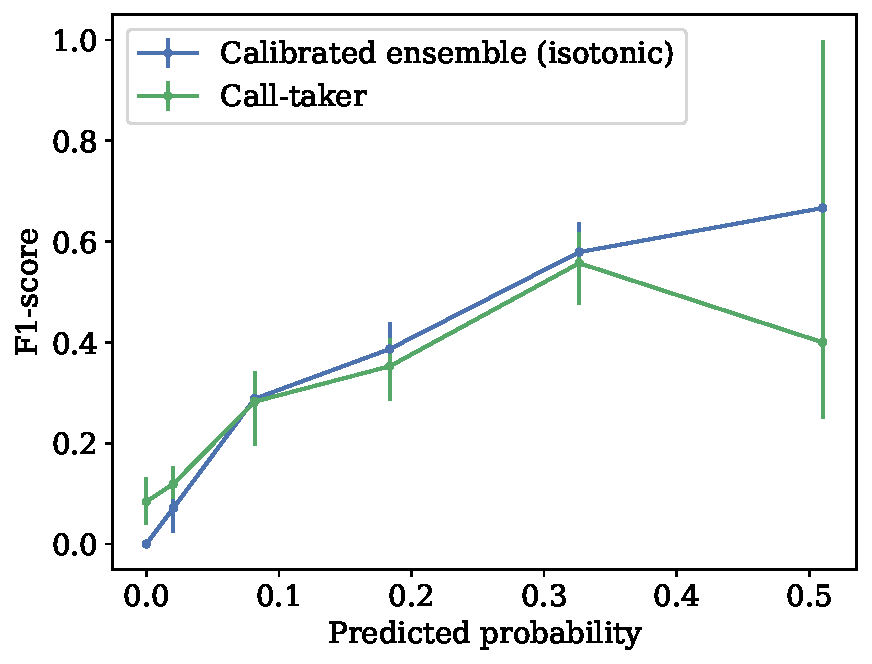
\includegraphics[width=1\columnwidth]{paper_retrospective_calibration_plots/f1_score_vs_predicted_probability_ensemble_calltaker_with_cis.pdf}
    \end{subfigure}
    \hfill
    \begin{subfigure}[c]{0.49\columnwidth}
        \centering
        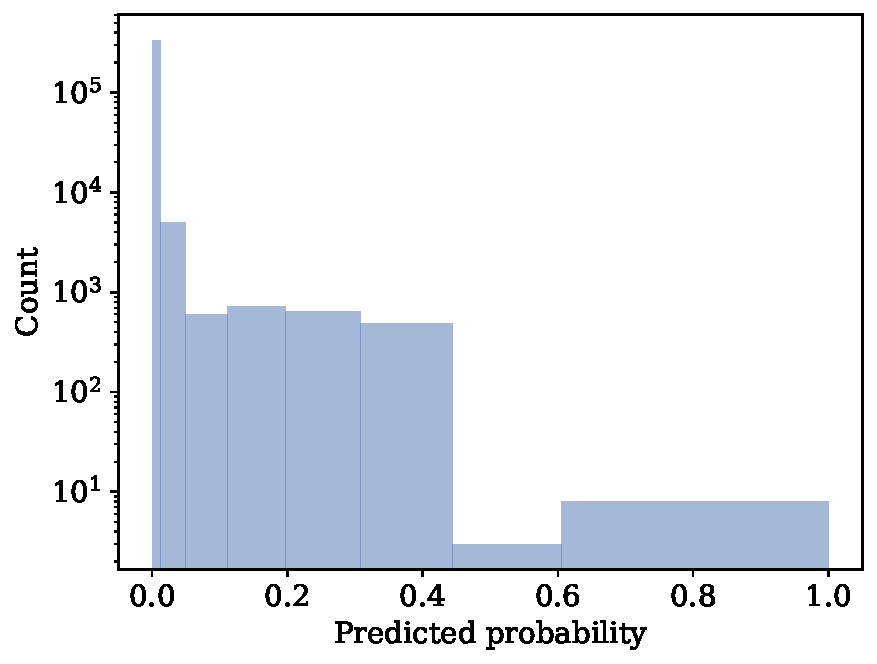
\includegraphics[width=1\columnwidth]{paper_retrospective_calibration_plots/predicted_probability_histogram.pdf}
    \end{subfigure}    
    \caption[Comparison of F1-score of stroke recognition ensemble and call-takers as function of predicted probability.]{ Comparison of the F1-score of the stroke recognition ensemble and call-takers. The F1-score is computed on subsets of the test dataset made by binning on the predicted probabilities of the calibrated ensemble. We see that the relative performance improvement of the ensemble over call-takers is higher towards more certain predictions. We use the ensemble that achieved the median F1-score reported in \cref{fig_retrospective:figure1-roc-curve} and \cref{tab_retrospective:table3-occlusion-analysis}.}
    \label{fig_discussion:retrospective-paper-f1-performance-vs-predicted-probability}
\end{figure}

Clinicians in intensive care units and emergency departments have been found to strongly agree that a singular focus on overall accuracy cannot alone ensure sustained trust in a model \cite{tonekaboni_what_2019}. Clinicians expect an alert to present a prediction that aligns with patient status. Despite expert-agreed thresholds for when alerts should be triggered, however, many alerts may not be aligned since class imbalance and ambiguous information in many predictive problems in healthcare can lead to models with relatively low predictive precision \parencite{umscheid_development_2015, cite14, cite15, wenstrup_retrospective_2023}. In turn, this is likely to lead to alarm fatigue \parencite{embi_evaluating_2012} and can undermine the sustained use and endorsement by clinicians of such systems \parencite{guidi_clinician_2015}. 
The stroke recognition ensemble presented in \cref{chp:paper-retrospective} is not exempt from this risk. With a precision of $24.9\%$ (95\% confidence interval $24.3-25.5\%$) it will on average be wrong three out of four times it predicts a stroke. This unfortunately risks alarm fatigue among its potential users, diminishing its effect in practice.

Calibrated probabilities in the alerts presented to users might be a way to alleviate the problem of alarm fatigue. They would allow users to discern between certain and uncertain predictions and also enable the system to present users only with predictions that have a minimum probability of being correct. Similar approaches have been suggested by clinicians and interviews indicate that predictive uncertainty is perceived by experts as a kind of explanation that complements the prediction \cite{tonekaboni_what_2019}. In \cref{fig_discussion:retrospective-paper-f1-performance-vs-predicted-probability} we show the F1-score of the ensemble model and the call-takers computed on subsets of the data created by binning the calibrated probabilities. We note that, as might be expected, both call-taker and ensemble model performance increase with increased model certainty. This indicates that selecting, based on certainty, which predictions to present to users might indeed help build trust in the system, reduce alarm fatigue, and ensure a practical impact. 
